To test our implementation of the algorithm, we simulated data with 50 covariates and 500 observations, where the covariates were sampled from a normal distribution with mean zero and variances 25, 5, and 0.4 sampled form a multinomial distribution with probability vector $(.05, .05, .9)$. Data was normalized to have mean zero and a standard deviation of one. No intercept was fit.\\

In general, we find that the algorithm requires careful attention to the step rate $\eta$, the number of time steps $m$, and the size of the minibatch for the stochastic gradient. While these parameters don't need to be calibrated precisely, they need to be on the right order of magnitude or the algorithm will not converge or mix poorly.

For the simulated data, we chose ... [mention parameters]

We can see that using the Hamiltonian Monte Carlo algorithm produced good mixing with energy decreasing downwards and converging:

\begin{figure}[H]
	\centering
	\begin{minipage}{0.45\textwidth}
		\centering
		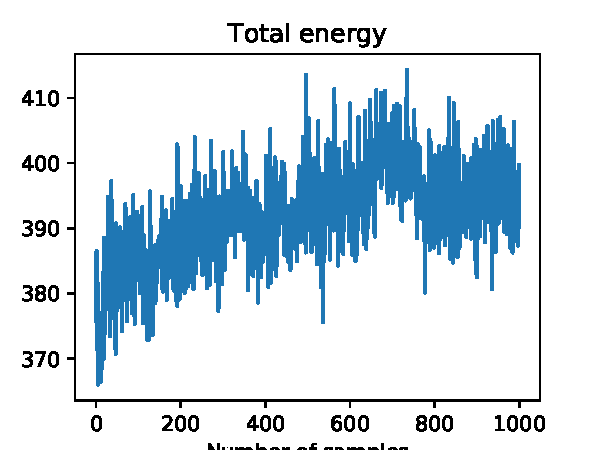
\includegraphics[width=0.9\textwidth]{hmc-energy-sim.pdf} % first figure 
	\end{minipage}\hfill
	\begin{minipage}{0.45\textwidth}
		\centering
		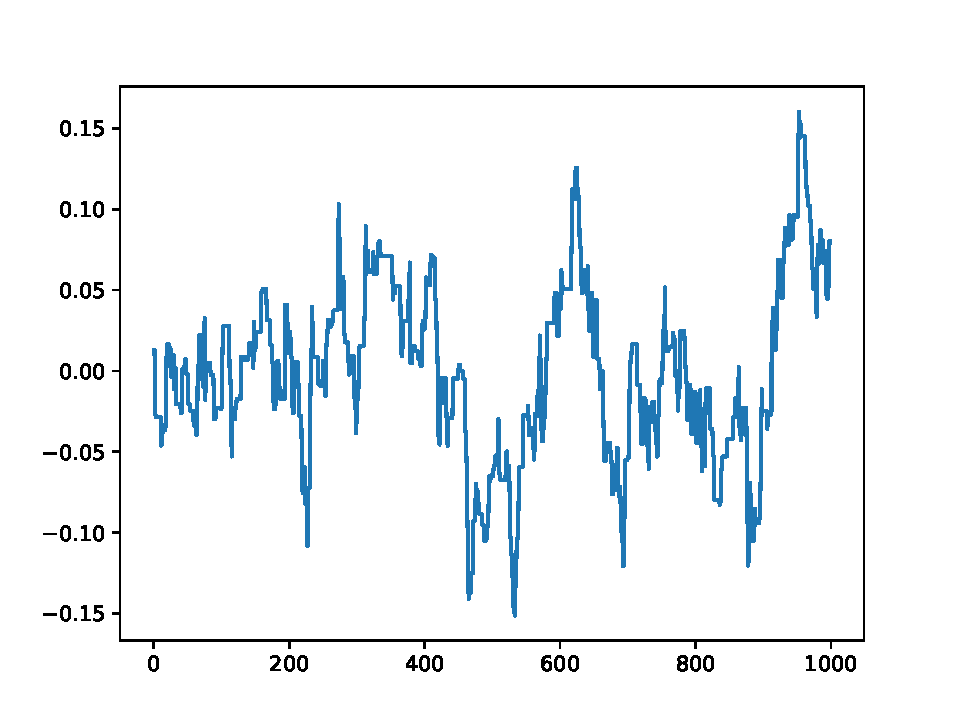
\includegraphics[width=0.9\textwidth]{hmc-trace-sim.pdf} % second figure 
	\end{minipage}
\end{figure}

We can see that using the Stochastic Gradient Hamiltonian Monte Carlo algorithm produced good mixing with energy decreasing downwards and converging:

\begin{figure}[H]
	\centering
	\begin{minipage}{0.45\textwidth}
		\centering
		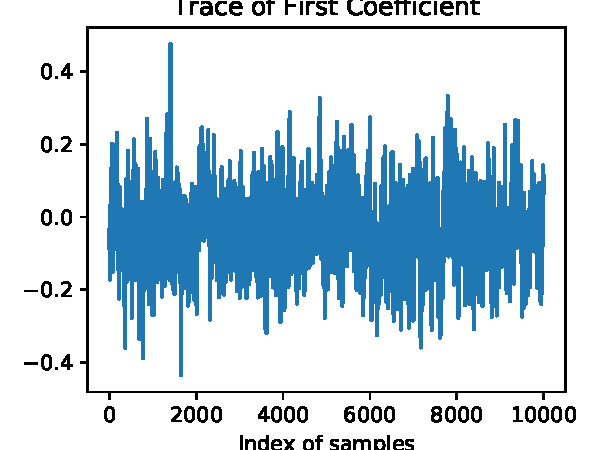
\includegraphics[width=0.9\textwidth]{sghmc-trace-sim.pdf} % first figure
	\end{minipage}\hfill
	\begin{minipage}{0.45\textwidth}
		\centering
		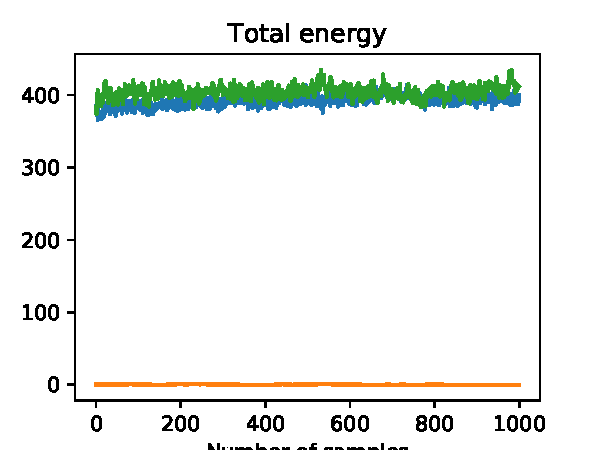
\includegraphics[width=0.9\textwidth]{sghmc-energy-sim.pdf} % second figure
	\end{minipage}
\end{figure}

We compared the coefficients produced by each algorithm to the MLE estimates to check for accuracy:

\begin{figure}[H]
	\centering
	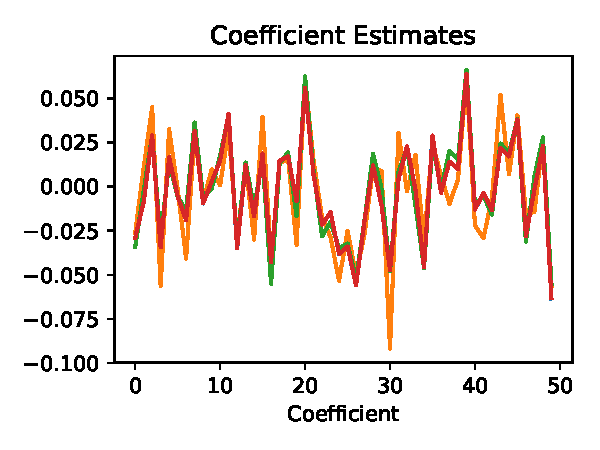
\includegraphics[width=0.45\textwidth]{coefs-sim.pdf}
\end{figure}

We see that all coefficients are fairly similar.